\subsection{Übung}
\subsubsection{}

At first, a sinusoidal sound signal with $L_p$ = \SI{60}{dB\ SPL}, a duration of \SI{1}{\s} and a frequency $f$ = \SI{1}{\kilo\Hz} was generated. This signal was sampled at a frequency $f_s$ of \SI{20}{\kilo\Hz}. To introduce the sound pressure level (SPL) into the signal the following derivation was developed. As reference sound pressure, the threshold of human hearing $p_0$ = \SI{20}{\micro\pascal} was chosen. $\hat{p}$ thereby indicates the peak value of the pressure wave, while $\tilde{p}$ is the effective value of the sinusoidal pressure amplitude.(Eq. \ref{eq:eff}) Simplistically, the static pressure component was neglected for further computations.

Solving equation \ref{eq:eff} and \ref{eq:l_p} after $\hat{p}$ results in the solution (\ref{eq:p_hat}). Following this, the final pressure wave could be computed in equation \ref{eq:p_wave} with the given parameters. A snippet from the wave is also shown in figure \ref{fig:signal}.
\begin{align}
    \tilde{p}\ &=\ \frac{\hat{p}}{\sqrt{2}} \label{eq:eff}\\
    L_p\ &=\ 20\ log\left(\frac{\tilde{p}}{p_0} \right) \label{eq:l_p}\\
    \hat{p}\ &=\ \sqrt{2}\ \cdot\ 10^{\frac{L_p}{20}}\ \cdot\ p_0 \label{eq:p_hat}\\
    p(t)\ &=\ \hat{p} \sin(2\pi f t) \label{eq:p_wave}
\end{align}
\begin{figure}[h] 
  \centering
  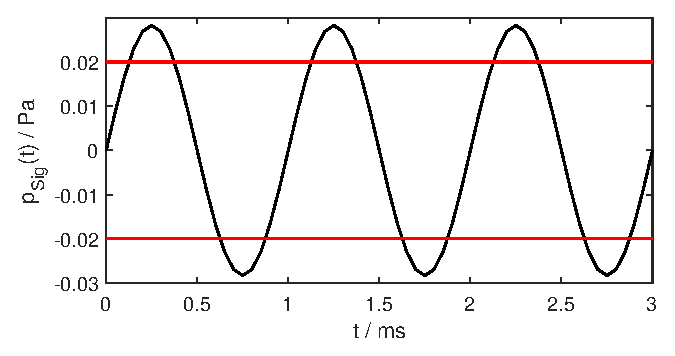
\includegraphics[width=.9\linewidth]{ue2/sig.eps} % oder statt scale auch [width=0.5\textwidth] für eine feste Größe
  \caption{Sinusoidal pressure signal for further analysis. The red lines indicate the RMS-SPL at \SI{60}{dB} and lie at $\approx$ 70 \% ($\frac{1}{\sqrt{2}}$) of the peak amplitude.}
  \label{fig:signal}
\end{figure}

\newpage

Subsequently, the acoustic pressure level was computed from the spectrum of the pressure wave from figure \ref{fig:signal}. We would assume a single peak slightly above \SI{60}{dB} at \SI{1}{\kilo\Hz} with decaying flanks in the frequency domain. This is proven by the plot in figure \ref{fig:pegel_fft}.
\begin{figure}[h] 
  \centering
  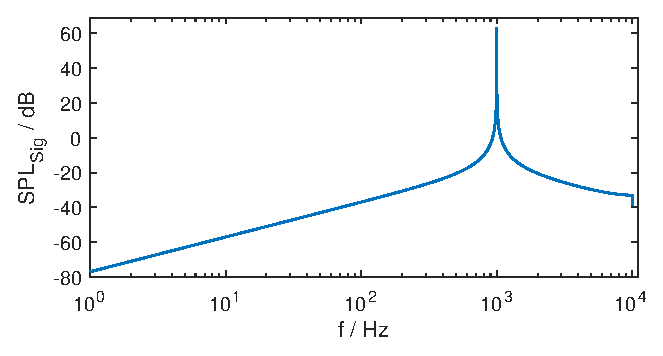
\includegraphics[width=.9\linewidth]{ue2/L_U_sig.eps} % oder statt scale auch [width=0.5\textwidth] für eine feste Größe
  \caption{Acoustic pressure level of the Fourier-transformed pressure wave from figure \ref{fig:signal}}.
  \label{fig:pegel_fft}
\end{figure}

\clearpage
\subsubsection{}
By playing the sound on the headphones, a cracking noise is noticeable in the beginning and the end of the signal. This happens due to the non differentiable step in the signal at both sides. To counteract this, start and end of the tone were filtered with the corresponding half a Blackman window to generate a fading-effect.

\begin{figure}[h] 
  \centering
  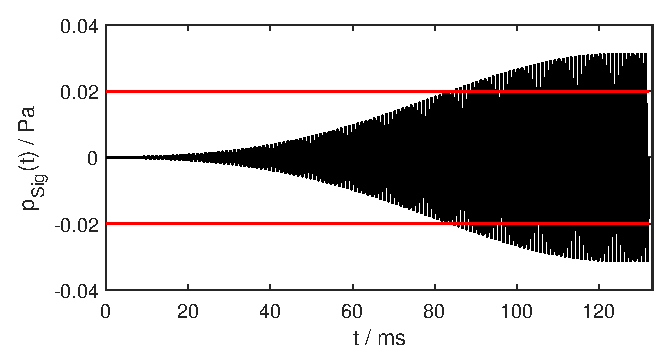
\includegraphics[width=.9\linewidth]{ue2/soundsig.eps} % oder statt scale auch [width=0.5\textwidth] für eine feste Größe
  \caption{Blackman - windowed sound signal for fading start and end to reduce the cracking noise. The red lines indicate the \SI{60}{dB SPL}.}
  \label{fig:sound}
\end{figure}



\clearpage
\subsubsection{}
In this exercise, two recorded audio signals with the word "Nuss" and the letter "w" (spoken "double-u") were loaded into the program and scaled to a RMS-SPL of \SI{60}{dB\ SPL}. Then, the corresponding spectrum of the SPL was computed. (Figs. \ref{fig:nuss_pegel} and \ref{fig:w_pegel}). 

Afterwards, both signals were A-weighted.(Figs.\ref{fig:nuss_a} and \ref{fig:w_a}) This filter is applied to convert the machine-measured loudness of a signal to the non-linear relative loudness perceived by humans. The particular "A" filter corresponds to the 40-phon Fletcher–Munson curve, which is considered to be the most accurate equal-loudness contour for human hearing.

The pressure level spectra were also evaluated for both signals. (Figs. \ref{fig:nuss_pegel_a} and \ref{fig:w_pegel_a}). In comparison to the levels of the unfiltered SPL, a clear dampening of frequencies below ($\approx$ \SI{10}{\Hz}) and above ($\approx$ \SI{20}{\kilo\Hz}) the absolute auditory threshold could be observed.
\clearpage
\begin{figure}[h] 
  \centering
  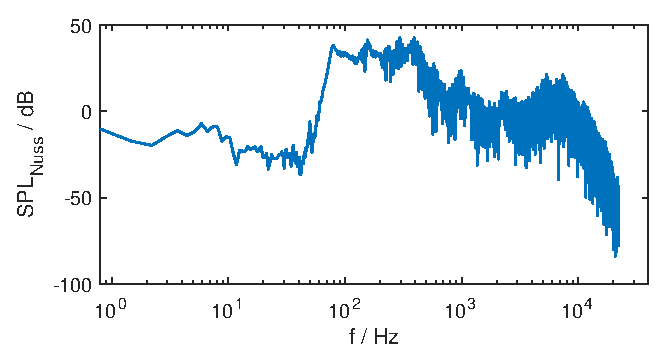
\includegraphics[width=.9\linewidth]{ue2/nuss_pegel.eps} % oder statt scale auch [width=0.5\textwidth] für eine feste Größe
  \caption{SPL spectrum of an audio record of the german word "Nuss".}
  \label{fig:nuss_pegel}
\end{figure}

\begin{figure}[h] 
  \centering
  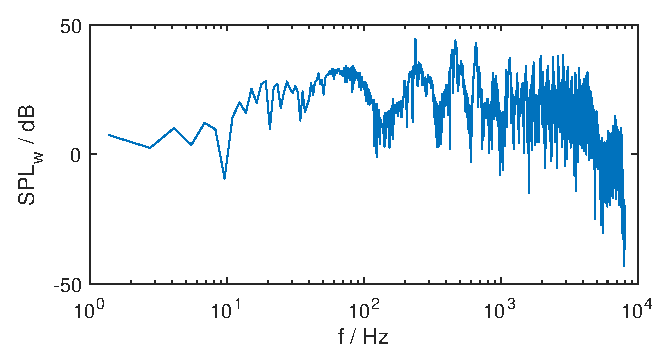
\includegraphics[width=.9\linewidth]{ue2/w_pegel.eps} % oder statt scale auch [width=0.5\textwidth] für eine feste Größe
  \caption{SPL spectrum of an audio record of the english letter "w".}
  \label{fig:w_pegel}
\end{figure}

\begin{figure}[h] 
  \centering
  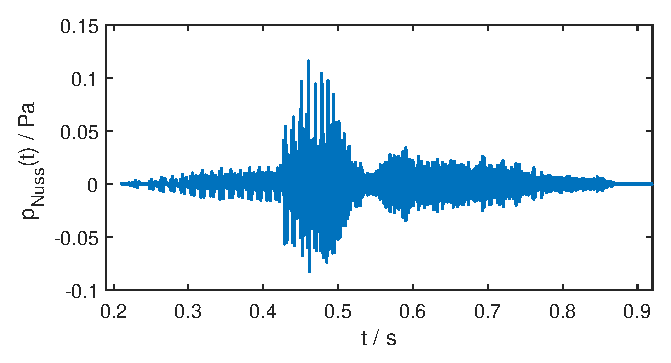
\includegraphics[width=.9\linewidth]{ue2/sa_nuss.eps} % oder statt scale auch [width=0.5\textwidth] für eine feste Größe
  \caption{A-weighted signal of an audio record of the german word "Nuss".}
  \label{fig:nuss_a}
\end{figure}


\begin{figure}[h] 
  \centering
  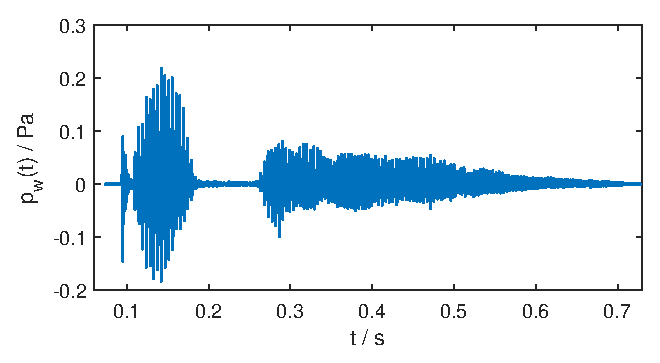
\includegraphics[width=.9\linewidth]{ue2/sa_w.eps} % oder statt scale auch [width=0.5\textwidth] für eine feste Größe
  \caption{A-weighted signal of an audio record of the english letter "w".}
  \label{fig:w_a}
\end{figure}

\begin{figure}[h] 
  \centering
  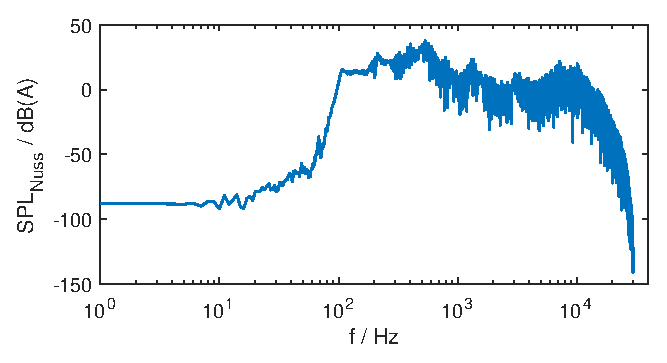
\includegraphics[width=.9\linewidth]{ue2/sa_nuss_pegel.eps} % oder statt scale auch [width=0.5\textwidth] für eine feste Größe
  \caption{A-weighted SPL spectrum of an audio record of the german word "Nuss".}
  \label{fig:nuss_pegel_a}
\end{figure}

\begin{figure}[h] 
  \centering
  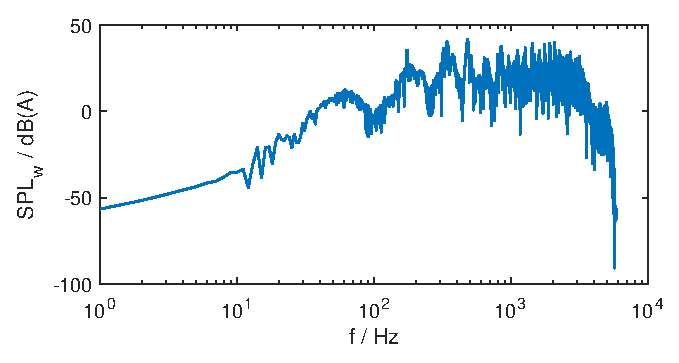
\includegraphics[width=.9\linewidth]{ue2/sa_w_pegel.eps} % oder statt scale auch [width=0.5\textwidth] für eine feste Größe
  \caption{A-weighted SPL spectrum of an audio record of the english letter "w".}
  \label{fig:w_pegel_a}
\end{figure}
\clearpage

\subsubsection{}
In the follwing, the audiosignals were plotted in a spectrogram (time x frequency x power). The dampening of the very high and very low frequencies by the A-filter can be oberved as black stripes at the top and bottom of the corresponding plots. (Figs. \ref{fig:nuss_spectro} vs. \ref{fig:a_nuss_spectro} and \ref{fig:w_spectro} vs. \ref{fig:a_w_spectro}).

For the word "Nuss", we can observe many frequency variations from letter to letter. The letter "N" can only be seen in very low frequencies with its harmonics above. "U" is then spoken in a slightly higher frequency band with more intense harmonics. In contrast, the hissing sound of the double "S" is a superposition of many medium-high-frequent components.

The letter "W" ("double-u") is constructed from more letters, which can be distinguished from the spectrogram. First, we can observe two mountain ranges from the parts "DOU" and "BL" with a small pause in between. "BL" then fades into the low frequent "U" component. Interestingly, "D" seems to range from low to high frequencies, while "OU" fades for above \SI{6}{\kilo\Hz}. "BL" is the first mountain after the short pause in the word and migrates to a unwritten "J"-like sound. The mountain raising from (\SI{2}{\kilo\Hz},\SI{300}{\milli\second}) to (\SI{5}{\kilo\Hz},\SI{450}{\milli\second}) and falling back to low frequencies from \SI{500}{\milli\second} to \SI{600}{\milli\second} account for the fade "BL" -> "J" and "J" -> "U". Similarly to "Nuss", "U" is then built only from low frequencies.

The parameters, with which the \textit{spectrogram()} function is called, mainly affect the sharpness resp. smoothness between time- and frequency-steps. For the following, a Blackman-window with a length of 256 and a maximal overlap of 220 samples for adjoining windows was chosen. Fewer overlap hereby accounts for sharper transitions between time-frequency bins. Another parameter to refine the plot result is to maximize the number of DFT-bins "nfft". This was set to the MATLAB internal maximum of 256. By not evaluating desired frequencies specifically, MATLAB chose appropriate spaced frequencies from 0 to $f_s/2$ itself.

\clearpage

\begin{figure}[t] 
  \centering
  \includegraphics[width=\linewidth]{ue2/nuss_spectro.eps} % oder statt scale auch [width=0.5\textwidth] für eine feste Größe
  \caption{Spectrogram of the word "Nuss".}
  \label{fig:nuss_spectro}
\end{figure}
\begin{figure}[b] 
  \centering
  \includegraphics[width=\linewidth]{ue2/a_w_nuss_spectro.eps} % oder statt scale auch [width=0.5\textwidth] für eine feste Größe
  \caption{A-weighted spectrogram of the word "Nuss".}
  \label{fig:a_nuss_spectro}
\end{figure}

\clearpage
\begin{figure}[t] 
  \centering
  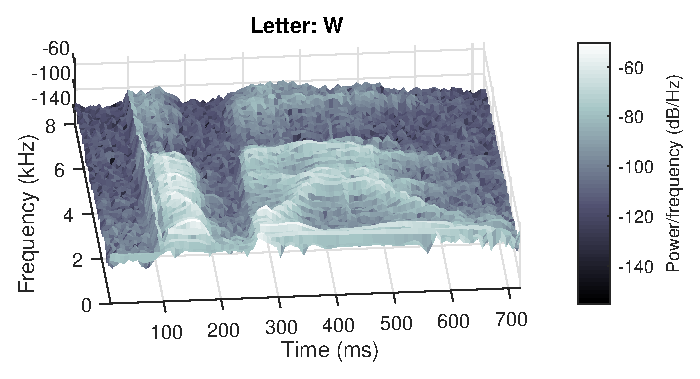
\includegraphics[width=\linewidth]{ue2/w_spectro.eps} % oder statt scale auch [width=0.5\textwidth] für eine feste Größe
  \caption{Spectrogram of the letter "double-u".}
  \label{fig:w_spectro}
\end{figure}

\begin{figure}[b] 
  \centering
  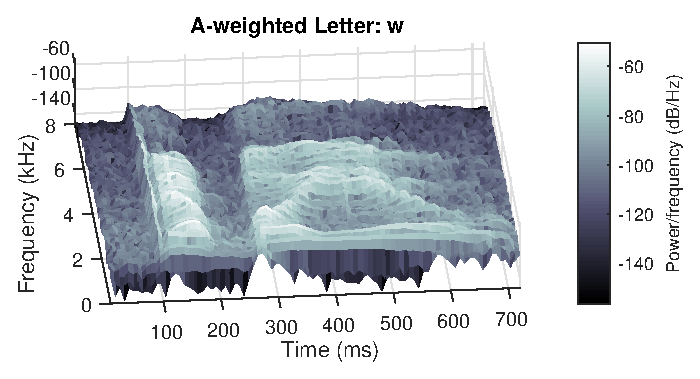
\includegraphics[width=\linewidth]{ue2/a_w_w_spectro.eps} % oder statt scale auch [width=0.5\textwidth] für eine feste Größe
  \caption{A-weighted spectrogram of the letter "double-u".}
  \label{fig:a_w_spectro}
\end{figure}